% rubber: set program xelatex
\documentclass[18pt]{beamer}

%{{{ Settings
\usetheme[english, titlepage0]{KIT}

%{{{ Packages
\usepackage{tikz}
\usepackage{xltxtra}
\usepackage{csquotes}
\usepackage{hyperref}
\usepackage[framemethod=tikz]{mdframed}
%}}}
%{{{ Fonts and colors
\setsansfont[Mapping=tex-text,
             BoldFont={* Semibold}]{Source Sans Pro}
\setmonofont[UprightFeatures={LetterSpace=-0.5}]{Inconsolata}

% TomorrowTheme: https://github.com/chriskempson/tomorrow-theme/blob/master/vim/colors/Tomorrow.vim
\definecolor{syntax-comment}{HTML}{8e908c}
\definecolor{syntax-keyword}{HTML}{8959a8}
\definecolor{syntax-number}{HTML}{eab700}
\definecolor{syntax-green}{HTML}{718c00}
\definecolor{syntax-red}{HTML}{c82829}

\setbeamercolor{section in toc}{fg=black!80}
%}}}
%{{{ TikZ styles
\usetikzlibrary{arrows, backgrounds, calc, trees, shapes, snakes}

\tikzset{
  commit/.style={
    circle, draw, color=black!75, fill=syntax-keyword!75,
    line width=1pt, minimum height=12pt
  },
  connection/.style={
    draw, ->, >=stealth, color=black!75, line width=.75pt
  }
}

\pgfdeclareimage[width=.36cm]{butthurt}{images/butthurt}

\newcommand\score[2]{
  \pgfmathsetmacro\pgfxa{#1+1}
  \begin{tikzpicture}[baseline=-3pt]
    \foreach \i in {1,...,#2} {
      \pgfmathparse{(\i<=#1?"1.0":"0.3")}
      \edef\starcolor{\pgfmathresult}
      \node[name=butthurt\i, opacity=\starcolor, inner sep=0pt] at (\i*3ex,0) {\pgfuseimage{butthurt}};
    }
  \end{tikzpicture}
}

\makeatletter
\tikzset{
  circle split part fill/.style  args={#1,#2}{%
    alias=tmp@name, % Jake's idea !!
    postaction={%
      insert path={
        \pgfextra{%
          \pgfpointdiff{\pgfpointanchor{\pgf@node@name}{center}}%
                       {\pgfpointanchor{\pgf@node@name}{east}}%
          \pgfmathsetmacro\insiderad{\pgf@x}
          \fill[#1] (\pgf@node@name.base) ([xshift=-\pgflinewidth]\pgf@node@name.east) arc
                            (0:180:\insiderad-\pgflinewidth)--cycle;
          \fill[#2] (\pgf@node@name.base) ([xshift=\pgflinewidth]\pgf@node@name.west)  arc
                            (180:360:\insiderad-\pgflinewidth)--cycle;
        }
      }
    }
  }
}
\makeatother
%}}}
%{{{ Environments
\makeatletter
\newenvironment{shell}[1][\linewidth]
  {\begin{mdframed}[
  skipabove=\topsep,
  skipbelow=\topsep,
  font=\ttfamily,
  linecolor=black!9,
  backgroundcolor=black!9,
  innertopmargin=6pt,
  innerbottommargin=6pt,
  innerleftmargin=6pt,
  innerrightmargin=6pt,
  userdefinedwidth=#1]}
  {\end{mdframed}}
\makeatother
%}}}
%{{{ Meta
\title{Distributed version control and why \emph{you} want to use it}
\author{M. Vogelgesang}
\subtitle{Matthias Vogelgesang}
\institute{Institute for Data Processing and Electronics}
\date{Oct.~17\textsuperscript{th} 2013}

\graphicspath{{../../common/}}

% \KITtitleimage{background.jpg}
%}}}

%}}}

\begin{document}
\maketitle

\section{Version Control}

\begin{frame}{Plead guilty!}
  It's easy to copy digital content, so why not re-create it over and over
  again?

  \begin{columns}[onlytextwidth]
    \visible<2->{
      \column{0.5\textwidth}
        \begin{figure}
          \centering
          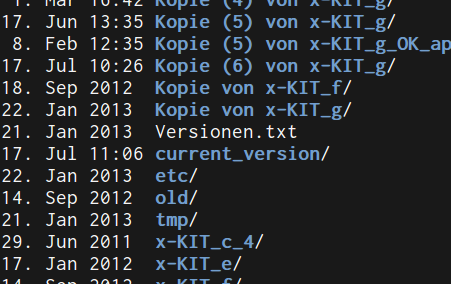
\includegraphics[width=4.5cm]{images/mrcs.png}
          \caption*{\enquote{One of these folders \emph{must} contain the latest
          version \ldots}}
        \end{figure}
    }

    \visible<3->{
      \column{0.5\textwidth}
        \begin{figure}
          \centering
          
\includegraphics[width=4.5cm]{images/reports.png}
          \caption*{\enquote{Here is the latest version of the
          proposal/paper/report.} --- \enquote{Thanks.}}
        \end{figure}
    }
  \end{columns}
\end{frame}
\begin{frame}{Obvious disadvantages}
  \begin{itemize}
    \item You lose track of what's going on
    \item No meta data about \emph{what} was changed \emph{when} by
      \emph{whom}
    \item Poor solution for collaboration
  \end{itemize}
\end{frame}
\begin{frame}{Version control to the rescue}
  Version controlled repository allow you to
  \begin{itemize}
    \item \emph{Track} files
    \item \emph{Commit} changes
    \item Share changes with others
    \item Roll-back to an earlier state
  \end{itemize}
\end{frame}

\section{Distributed Version Control}

\begin{frame}{Distributed version control}
  \begin{block}{What's wrong with CVS/SVN/\ldots?}
    \begin{itemize}
      \item Nothing per se but\ldots
      \item They require a central server instance
        \begin{itemize}
          \item Interaction with a repository can be painfully slow
          \item Setup and maintenance issues
        \end{itemize}
    \end{itemize}
  \end{block}

  \begin{block}{How can DVCS help?}
    \begin{itemize}
      \item Every developer has a clone of the \emph{full} repository
        \begin{itemize}
          \item Blazingly fast operations
          \item Without a server, working offline becomes possible
          \item Easier initial setup
        \end{itemize}
      \item DVCS are built around the idea of sharing
        \begin{itemize}
          \item Easier branching
          \item Usually easier merging
        \end{itemize}
    \end{itemize}
  \end{block}
\end{frame}
\begin{frame}{Distributed version control \emph{systems}}
  Mercurial, Bazaar, SVK, Monotone, BitKeeper, \textbf{Git}, Darcs, Fossil, GNU
  arch, Arx, Plastic SCM
\end{frame}
\begin{frame}{Why Git?}
  \begin{columns}[T,onlytextwidth]
    \column{0.5\textwidth}
      \begin{block}{Pros}
        \begin{itemize}
          \item De-facto standard for open source software
          \item Probably the fastest DVCS out there
          \item SourceForge lost its sex appeal against GitHub
        \end{itemize}

      \end{block}

      \begin{block}{Cons}
        \begin{itemize}
          \item Command line interface feels can be a bit inconsistent
          \item Git is a toolbox with much freedom and little limits
        \end{itemize}
      \end{block}
    \column{0.5\textwidth}
      \centering
      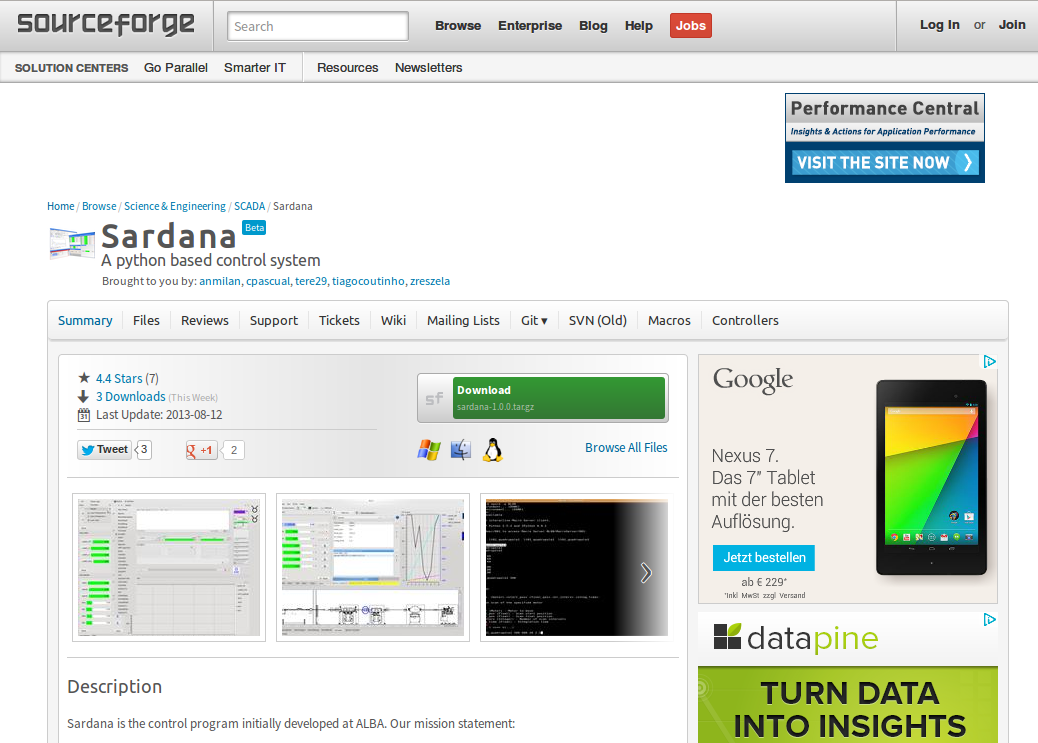
\includegraphics[width=4.0cm]{images/sf.png}
      \vspace{1em}
      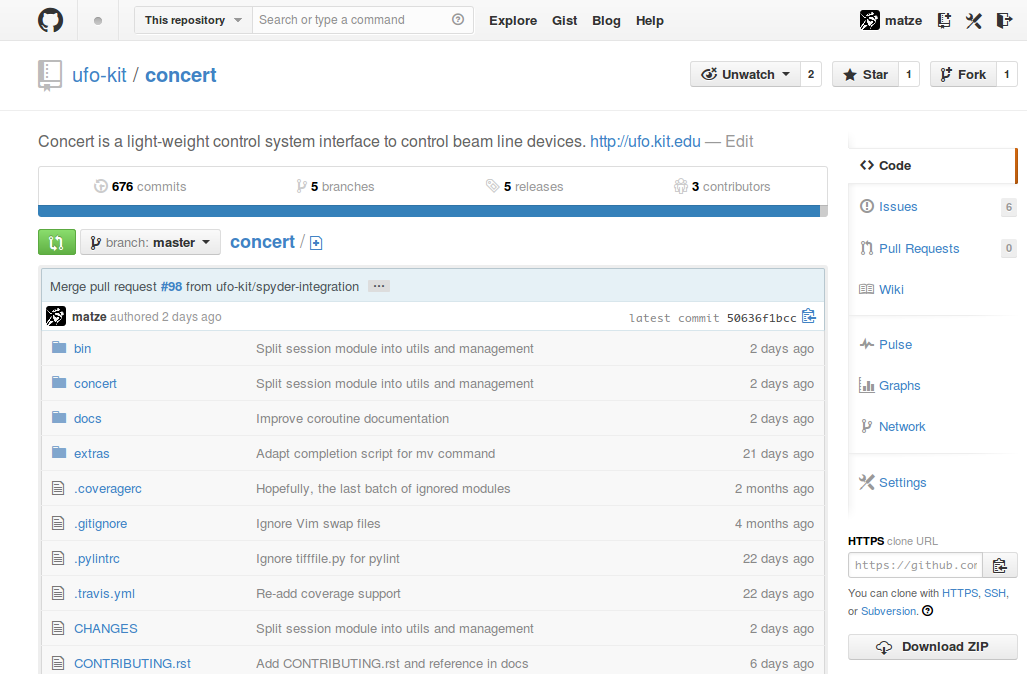
\includegraphics[width=4.0cm]{images/github.png}
  \end{columns}
\end{frame}

\section{Hands-on introduction}

\begin{frame}{}
  \begin{center}
    \huge\bfseries
    \textcolor{KITblack50}{Git basics}
  \end{center}
\end{frame}

\begin{frame}{Getting started}
  \begin{block}{Installation}
    \begin{itemize}
      \item Debian/Ubuntu: \texttt{apt-get install git-core}
      \item openSUSE/SLES: \texttt{zypper install git-core}
      \item Fedora/RHEL/CentOS/SL: \texttt{yum install git}
      \item Mac: \texttt{port install git-core} or install from
      \url{http://git-scm.com/download/mac}
      \item Windows: install from \url{http://git-scm.com/download/win}
    \end{itemize}
  \end{block}
\end{frame}
\begin{frame}{Creating a new repository}
  In the working directory of your project, type
  \begin{shell}
    \$ git init
  \end{shell}
  \begin{block}{No server?}
    \begin{itemize}
      \item \emph{Everything} is stored locally in the hidden \texttt{.git}
        sub-directory
      \item Synchronizing changes with a remote location happens in a separate
        step
    \end{itemize}
  \end{block}
\end{frame}
\begin{frame}{What' going on?}
  \begin{shell}
    \$ git status
  \end{shell}
\end{frame}
\begin{frame}{Tracking files}
  \begin{shell}
    \$ git add
  \end{shell}
\end{frame}
\begin{frame}{Committing changes}
  \begin{shell}
    \$ git commit
  \end{shell}
\end{frame}
\begin{frame}{Recording changes}
  At some point changes need to be \emph{staged} and \emph{committed}
  \begin{shell}
\$ vi paper.tex\\
\$ git add paper.tex\\
\$ git commit
  \end{shell}
  or in one go
  \begin{shell}
    \$ git commit -a
  \end{shell}
\end{frame}
\begin{frame}{Excursion: File states}
  \begin{figure}
    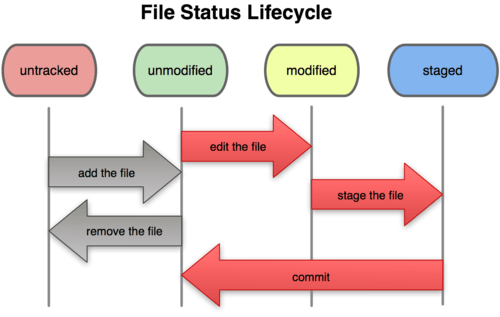
\includegraphics[width=9cm]{images/files}
    \caption{from Scott Schacon's \enquote{Pro Git} CC-BY-NC-SA 3.0}
  \end{figure}
\end{frame}
\begin{frame}{Logged information}
  To see the most recent changes in a pager, use

  \begin{shell}
    \$ git log
  \end{shell}

  \begin{block}{GUIs for the faint-hearted}
    Have a look at gitg, gitk, giggle, tig \ldots
  \end{block}
\end{frame}
\begin{frame}{Branches}
  \begin{columns}[onlytextwidth]
    \column{0.7\textwidth}
      If you want to explore an idea without messing with your pristine
      original work, you can create a branch off of it \ldots

      \begin{shell}
        \$ git branch fancy-idea\\
        \$ git checkout fancy-idea
      \end{shell}

      \visible<2->{
        and commit changes related to that idea
        \begin{shell}
          \$ git commit \ldots
        \end{shell}
      }

      \visible<3->{
        Once, committed you can switch back and forth
        \begin{shell}
          \$ git checkout master\\
          \$ git commit \ldots
        \end{shell}
      }

      \visible<4->{
        Branches are cheap, so don't bother creating as many as you like.
      }

    \column{0.3\textwidth}
      \centering
      \begin{tikzpicture}
        \node[commit, circle, draw] (root) at (0,0) {};
        \visible<3->{
          \node[commit] (c1) at (0,1.5) {};
        }

        \visible<2->{
          \node[commit] (b1) at (1,1) {};
          \node[commit] (b2) at (1,2) {};
          \draw (root.north) edge[connection, out=90, in=270] (b1.south);
          \draw[connection] (b1) -- (b2);
        }

        \visible<3->{
          \draw[connection] (root) -- (c1);
        }
      \end{tikzpicture}
  \end{columns}
\end{frame}
\begin{frame}{Merging changes}
  \begin{columns}[onlytextwidth]
    \column{0.7\textwidth}
      If your changes are ready for prime time, merge them into your master branch:

      \visible<2->{
        \begin{shell}
          \$ git checkout master\\
          \$ git merge fancy-idea
        \end{shell}

        In this case, a \emph{merge commit} will be created.
      }

      \visible<3->{
        \begin{block}{Removing branches}
        If merging was successful, the old branch can be removed

        \begin{shell}
          \$ git branch -D fancy-idea
        \end{shell}
        \end{block}
      }

    \column{0.3\textwidth}
      \centering
      \begin{tikzpicture}
        \node[commit, circle, draw] (root) at (0,0) {};
        \node[commit] (c1) at (0,1.5) {};
        \node[commit] (b1) at (1,1) {};
        \node[commit] (b2) at (1,2) {};

        \draw (root.north) edge[connection, out=90, in=270] (b1.south);
        \draw[connection] (root) -- (c1);
        \draw[connection] (b1) -- (b2);

        \visible<2->{
          \node[commit] (c2) at (0,3) {};
          \draw (b2.north) edge[connection, out=90, in=270] (c2.south);
          \draw[connection] (c1) -- (c2);
        }
      \end{tikzpicture}
  \end{columns}
\end{frame}
\begin{frame}{Collaborating with others}
  \begin{itemize}
    \item Until now, everything happened on our local machine
    \item To let others see you changes, you must setup a \emph{remote} and
      associate a local branch with a remote branch
  \end{itemize}
\end{frame}
\begin{frame}{Git best practices}
  \begin{itemize}
    \item Write good commit messages and keep 50/70 limits
    \item Rebase feature branches against master before merging
    \item Think twice before running \texttt{git commit -a}
  \end{itemize}
\end{frame}

\section{Advanced Git features}

\begin{frame}{}
  \begin{center}
    \huge\bfseries
    \textcolor{KITblack50}{Advanced Git}
  \end{center}
\end{frame}

\begin{frame}{Manipulating the Git object database}
  If you collaborate heavily with your peers, you'll want to have a
  \enquote{clean} history of changes, e.g.

  \begin{itemize}
    \item Concise commit messages
    \item One commit per logical change
    \item A series of commits leading to a bigger change
  \end{itemize}

  But: \emph{never} rewrite the history of changes that are already published or
  the Git gods will bring sorrow
\end{frame}
\begin{frame}{Fixing commit messages}
  \begin{shell}
    \$ git commit --amend
  \end{shell}
\end{frame}
\begin{frame}{Avoiding merge bubbles}
  \begin{columns}[onlytextwidth]
    \column{0.7\textwidth}
    When merging two branches that developed individually, you'll end up with a
    merge commit. You can avoid this situation by rebasing one branch on top of
    the other and fast-forward the merging with
      \begin{shell}
        \$ git checkout some-feature\\
        \$ git rebase master\\
        \$ git checkout master\\
        \$ git merge some-feature
      \end{shell}

    \column{0.3\textwidth}
      \centering
      \begin{tikzpicture}
        \node[commit, circle, draw] (root) at (0,0) {};
        \node[commit] (c1) at (0,1.5) {};
        \node[commit] (b1) at (1,1) {};
        \node[commit] (b2) at (1,2) {};
        \node[commit] (c2) at (0,3) {};

        \draw (root.north) edge[connection, out=90, in=270] (b1.south);
        \draw (b2.north) edge[connection, out=90, in=270] (c2.south);
        \draw[connection] (root) -- (c1);
        \draw[connection] (c1) -- (c2);
        \draw[connection] (b1) -- (b2);
      \end{tikzpicture}
  \end{columns}
\end{frame}
\begin{frame}{Partial staging}
  Sometimes, you made changes that are logically two different entities.
  However, good Git citizens have a clean history, so use:

  \begin{shell}
    git add -p/--patch
  \end{shell}
\end{frame}
\begin{frame}{Re-writing the history}
  \begin{columns}[onlytextwidth]
    \column{0.7\textwidth}
      Manipulate the change history by rebasing using the
      \texttt{-i/--interactive} switch

      \begin{itemize}
        \item \visible<2->{Drop commits}
        \item \visible<3->{Re-order commits}
        \item \visible<4->{Squash several commits into one}
        \item \visible<5->{Edit commits}
      \end{itemize}

      \visible<6->{
        \begin{shell}
        \$ git rebase -i HEAD\textasciitilde 4
        \end{shell}
      }

    \column{0.3\textwidth}
      \centering
      \begin{tikzpicture}
        % Drop commits
        \visible<1>{
          \node[commit] (c1) at (0,0) {};
          \draw[connection] (c1) -- (c2);
        }

        \visible<2->{
          \node[commit, opacity=0.5] (c1) at (0,0) {};
        }

        % Re-order commits
        \visible<1-2>{
          \node[commit, fill=syntax-number] (c2) at (0,1) {};
          \node[commit, fill=syntax-green!50] (c3) at (0,2) {};
        }

        \visible<3->{
          \node[commit, fill=syntax-green!50] (c2) at (0,1) {};
          \node[commit, fill=syntax-number] (c3) at (0,2) {};
          \path[connection, opacity=0.5] (c2.west) edge [bend left] (c3.west);
        }

        % Squash commits
        \visible<1-3>{
          \node[commit, fill=KITgreen50] (c5) at (0,4) {};
          \node[commit, fill=KITyellow50] (c4) at (0,3) {};
          \draw[connection] (c4) -- (c5);
        }

        \visible<4->{
          \node[shape=circle split, commit,
                circle split part fill={KITgreen50,KITyellow50}] (c4) at (0,3)
              {\nodepart{lower}};
        }

        \draw[connection] (c2) -- (c3);
        \draw[connection] (c3) -- (c4);
      \end{tikzpicture}
  \end{columns}
\end{frame}

\section{Beyond Source Control}

\begin{frame}{Managing large files}
  \begin{itemize}
    \item Managing big binary data is not recommended
    \item git-annex
    \item Nerd factor:\score{4}{5}
  \end{itemize}
\end{frame}
\begin{frame}{Bug tracking}
  \begin{itemize}
    \item ticgit, Fossil
    \item Nerd factor:\score{4}{5}
  \end{itemize}
\end{frame}
\begin{frame}{Blogging}
  \begin{itemize}
    \item GitHub pages
    \item Nerd factor:\score{2}{5}
  \end{itemize}
\end{frame}
\begin{frame}{Wiki}
  \begin{itemize}
    \item Based on Markdown: Gollum
    \item Nerd factor:\score{3}{5}
  \end{itemize}
\end{frame}
\begin{frame}{Backups}
  \begin{itemize}
    \item Bup
    \item Nerd factor:\score{2}{5}
  \end{itemize}
\end{frame}
\begin{frame}{Deployment}
  \begin{itemize}
    \item Using post-receive hooks
    \item Nerd factor:\score{1}{5}
  \end{itemize}
\end{frame}
\begin{frame}{Text-based slides}
  \begin{itemize}
    \item git-slides (together with Vim)
    \item Nerd factor:\score{5}{5}
  \end{itemize}
\end{frame}


\section{Appendix}

\begin{frame}{Further reads}
  \begin{columns}[T,onlytextwidth]
    \column{0.7\textwidth}
      \begin{itemize}
        \item \texttt{\$ man git} \ldots just kidding
        \item Free Pro Git book at \url{git-scm.com/book}
        \item Different aspects from beginners to pros: \url{gitready.com}
        \item Git cheat sheet: \url{ndpsoftware.com/git-cheatsheet.html}
        \item Interactive walkthrough: \url{gitimmersion.com}
      \end{itemize}

    \column{0.3\textwidth}
      \centering
      
\includegraphics[width=1.5cm]{images/pro-git}
      \vspace{2em}
      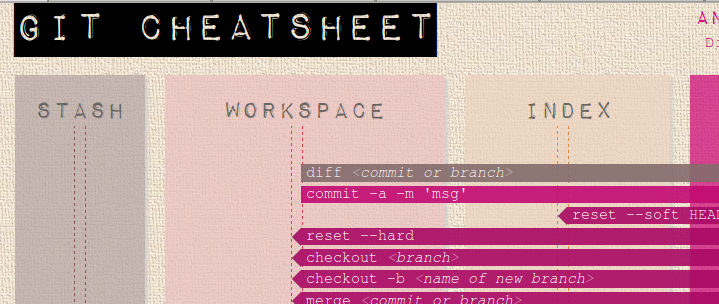
\includegraphics[width=3cm]{images/gcs}
  \end{columns}
\end{frame}

\begin{frame}{Conclusion}
  \begin{itemize}
    \item Use a distributed version control system, it \emph{will} help
    \item Clone these slides from \url{github.com/matze/kseta-dvsc-talk}
  \end{itemize}
\end{frame}

\end{document}

% vim:sw=2
